\chapter{Fundamentação Teórica}

\section{Modelagem de Processos}

Segundo \citeonline{katsuhiro2010}, a dinâmica de muitos sistemas mecânicos, elétricos, térmicos, entre outros pode ser descrita em termos de equações diferenciais. Estas equações são obtidas pelas leis físicas que o regem, como a equação Bernoulli para dinâmca de fluidos. Para modelar um sistema por tais equações, levanta-se o nível de detalhes esperado, já que nem todas as variáveis de uma função tem impacto significativo na sua resposta. Um exemplo deste cenário seria a resistência do ar para corpos em queda livre, em alturas pequenas.

De acordo com \citeonline{Lathi2007}, um sistema, após modelado, pode traduzir-se em um sistema linear ou não linear. Um sistema é dito linear se o princípio da superposição se aplicar a ele. Este princípio afirma que a resposta produzida pela perturbação simultânea de mais de uma entrada é a soma cada resposta se calculada individualmente. Isto possibilita solucionar equações complexas a partir do cálculo de partes da mesma, simplificando a solução.

Segundo \citeonline{katsuhiro2010}, uma forma comum de representação de um sistema linear invariante no tempo é pelas chamadas funções de transferências. Sendo $y(t)$ a função que descreve uma das saídas de um processo, e $x(t)$ uma das entradas, a função de transferência $G(s)$ traduz a influência de x em y. Este formato sempre relaciona uma saída a uma entrada, e é sempre representado pela razão entre a transformada de Laplace da primeira sobre a segunda, ou:
\begin{equation}
\frac{\mathcal{L}(y)}{\mathcal{L}(x)} = \frac{y{(s)}}{x(s)}
\end{equation}

\subsection{Linearização de sistemas}

Enquanto que sistema lineares tem propriedades que facilitam sua modelagem, de acordo com \citeonline{corripio2006}, sistemas não lineares não possuem técnicas tão diretas para analisar suas dinâmicas. Assim, podem ser empregadas neles trasformações para sistemas lineares equivalentes.

Uma delas é a chamada linearização, que emprega a série de Taylor, truncanda no segundo termo, ou
\begin{equation}
f(x_1, x_2, .. , x_n) \simeq f({x_1}_0, {x_2}_0, ..., {x_3}_0) + \bigg( \sum_{i=1}^n \frac{df}{dxi}\left.\right|_{x_i = {x_i}_0} ({x_i} - {x_i}_0) \bigg)
\end{equation}
, sendo $x_i$ os parâmetros da função descritiva $f$, e $({x_i}_0)$ um ponto de operação. Obtém-se, assim, uma função linearizada em torno de um determinado ponto do processo . Quanto mais as variáveis do sistema linearizado se afastarem deste ponto de operação, maior será o erro deste sistema, em relação ao sistema gerador não linear.

\section{Controladores}

Segundo \citeonline{Lourenco2007}, não é possível determinar o tipo de controlador a se usar num determinada processo. Idealmente, o controlador mais simples, que satisfaça a "resposta desejada" deve ser ser escolhido. Porém, a escolha depende também das condições de operação do sistema e de performance, como o erro estacionário máximo, e o tempo de estabelecimento permitido.

%Mantendo-se neste raciocínio, serão comparados dois controladores distintos neste caso de teste. No primeiro caso, o sistema será linearizado em torno de um ponto de operação e o resultado será utilizado para sintonizar um controlador PID. Em seguida o controlador será acoplado ao sistema. No segundo caso, um controlador mais simples será empregado, o chamado LQR, sintonizado por uma equação matemática, descrita na sua respectiva seção neste documento.

\citeonline{corripio2006} descrevem o controle por realimentação como o emprego de um controlador que monitora uma variável (a variável controlada do processo), compara o valor lido com o valor desejado, o \emph{setpoint}, e computa o sinal de controle a ser enviado para o sistema, através de uma variável manipulada.

\subsection{PID}

Segundo \citeonline{katsuhiro2010}, a utilidade dos controladores do tipo PID (Proporcional, Integral e Derivativo) está na sua aplicabilidade geral à maioria dos sistemas. Por conta disto, é um controlador bem popular. Ele recebe como sinal o erro $e$ de um sistema, que é a diferença entra o valor da variável controlada e seu setpoint. A partir disto, calcula o sinal de controle como:
\begin{equation}
u(t) = K_p e(t) + K_i \int e(t) + K_d \frac{de(t)}{dt}
\label{eq_PID}
\end{equation}
, a partir de seus ganhos $K_p$, $K_i$ e $K_d$ (proporcional, integral, derivativo).

Ainda de acordo com \citeonline{katsuhiro2010}, a definição dos ganhos de um controlador é um processo chamado sintonia, e pode ocorrer por vários métodos. Para um PID, exemplificam-se Ziegler-Nichols, otimização e resposta em frequência. \citeonline{corripio2006} descrevem um outro método, denominado síntese: dada uma função de transferência conhecida $P(s)$ de primeira ordem para um determinado processo, a função de transferência entre o controlador e seu sinal de controle será, em malha fechada (Figura \ref{img_exemplo_processo}):
\begin{equation}
C(s) = \frac{u(s)}{e(s)} = \frac{1}{P(s)} \frac{1}{\tau_c s}
\end{equation}
, com $\tau_c$ sendo o único parâmetro de sintonização, e representando o tempo que o sistema controlado deve levar até atingir 62,3\% do seu estado estacionário. Assim, se 
\begin{equation}
P(s) = \frac{G}{\tau s + 1}
\end{equation}
, então
\begin{equation}
C(s) = K_p + K_i \frac{1}{s} = \frac{\tau}{G \tau_c} + \frac{1}{G \tau_c} \frac{1}{s}
\label{sintese_controlador}
\end{equation}
, sendo $\tau$ e $G$ o tempo de resposta e o ganho natural do sistema, respectivamente.

\begin{figure}[hbt]
	\centering
	\caption{Processo 1x1 com feedback e controlador}
	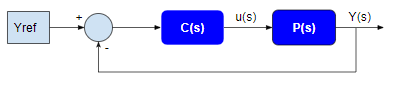
\includegraphics[width=0.8\textwidth]{exemplo_processo}
	\label{img_exemplo_processo}
\end{figure}

\subsection{LQR}

O Regulador Linear Quadrático, ou LQR, é um controlador de sintonia mais simples que o PID. Ele realiza um controle regulatório, ou seja, seu setpoint é sempre a origem (todos os estados e entradas em zero). Quanto à sua sintonia, segundo \citeonline{pythoncontrol}, o controlador recebe uma matriz $Q$ e uma matriz $R$, que atribuem pesos, respectivamente, aos estados e às entradas do sistema. Tomando um sistema genérico em espaço de estados:
\begin{equation}
\dot{x}(t) = A.x(t) + B.u(t)
\end{equation}
sendo $\dot{x}(t)$ as derivadas dos estados, $x(t)$ os estados, $A$ a matriz de estado, $u(t)$ as entradas e $B$ a matriz de entrada; o LQR aplicado será sintonizado de forma a minimizar a função quadrada de custo $J$ \ref{lqr_cost_func}:
\begin{equation}
J = \int_{0}^{\inf}(x'Qx + u'Ru)dt
\label{lqr_cost_func}
\end{equation} 

Segundo \cite{argentim2013}, a função de controle por realimentação $u$, para o caso do LQR, é representada pela equação \ref{lqr_generic_control_func}:
\begin{equation}
u = -Kx(t)
\label{lqr_generic_control_func}
\end{equation}
sendo $K$ a matriz de ganho do feedback dos estados.

Logo, em suma, a sintonia do LQR se dá ao encontrar a matriz $K$ que minimize a função de custo da equação \ref{lqr_cost_func}.

\section{SCADA}

De acordo com \citeonline{Martins2007}, os sistemas supervisórios podem ser considerados como o nível mais alto de IHM, pois mostram o que está acontecendo no processo e permitem ainda que se atue neste. A evolução dos equipamentos industriais, com a introdução crescente de sistemas de automação industrial, tornou complexa a tarefa de monitorar, controlar e gerenciar esses sistemas. 

Sistemas SCADAs são responsáveis por buscar informações de controladores e equipamentos diversos de automação, e manipular estas informações de acordo com o que foi programado. As aplicações mais simples se constituem na visualização dinâmica destes dados através de mostradores, cores, escalas, entre outros objeto gráficos em telas pré programadas. Uma estratégia, por exemplo, é a de literalmente desenhar todo um sistema produtivo através imagens já embutidas na biblioteca do software editor, e incluir nela todas as medições acessíveis, mapeando-as por onde se encontram no desenho. Outra seria a deagrupar as informações por temática, e mostrar diversas telas menos detalhadas, que alternem entre si de acordo com um temporizador interno. A Figura \ref{img_supervisorio_exemplo} ilustra um exemplo de tela para um sistema supervisório.

\begin{figure}[hbt]
	\centering
	\caption{Tela exemplo de um sistema supervisório}
	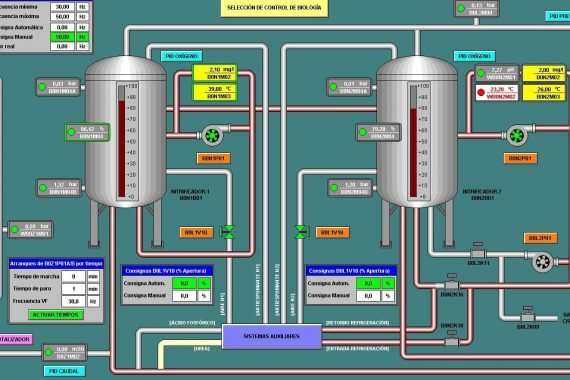
\includegraphics{Supervisorio_exemplo}
	Fonte: \href{https://www.agaads.com/service/scada-system/}{https://www.agaads.com/service/scada-system/}
	\label{img_supervisorio_exemplo}
\end{figure}

Por ser executado geralmente em um computador comum, a palavra chave de um sistema supervisório é flexibilidade. Um sistema SCADA deve ser capaz de se comunicar por diversos protocolos com diversos dispositivos, e adicionalmente disponibilizar os valores lidos para outros usuários, não somente os que têm acesso às telas. Isto se relaciona com o conceito já mencionado de software livre, descrito por \citeonline{junior2019}. Por possuir estas funcionalidades, software SCADAs ultrapassam o nível 2 na pirâmide de automação (Figura \ref{img_piramide_automacao}), chegando ao nível de supervisão da produção, pois agrupa as informações de diversos controladores e sensores em um só local, e gera suporte para ações de gerência.

\begin{figure}[hbt]
	\centering
	\caption{Pirâmide da automação}
	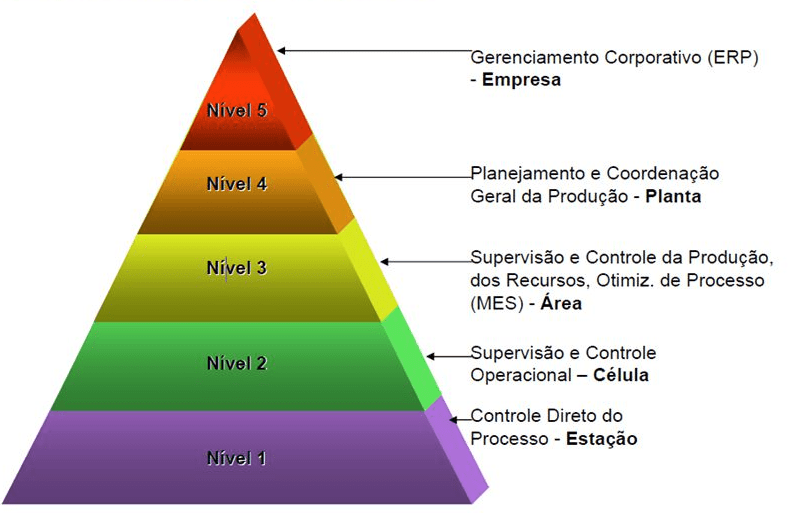
\includegraphics[width=0.8\textwidth]{piramide_automacao}
	Fonte: \href{https://www.logiquesistemas.com.br/blog/piramide-de-automacao-industrial/attachment/354/}{https://www.logiquesistemas.com.br/blog/piramide-de-automacao-industrial/attachment/354/}
	\label{img_piramide_automacao}
\end{figure}

Segundo \citeonline{Roggia2016}, dentre os principais benefícios do uso de sistemas de supervisão podem-se citar: informações instantâneas, redução no tempo de produção, redução no custo de produção, precisão das informações, detecção de falhas, aumento da qualidade e aumento da produtividade.

\section{Comunicação Serial}

Comunicação serial é um meio simples de dois equipamentos trocarem informação em formato de uma série de bits. De acordo com \citeonline{Bolton2015}, ela se dá através de um único cabo ou pino, transmitindo apenas um bit de cada vez. Apesar disto significar uma velocidade menor de envio de dados, a comunicação serial possui baixo custo, sendo popularmente utilizada na transmissão de dados por longas distâncias.Ainda existem outras tecnologias, como a chamada comunicação paralela, que utilizam mais canais de comunicação e podem portanto transmitir vários bits simultaneamente.

Segundo \citeonline{Mazidi2016}, existem dois tipos de comunicação serial: assíncrona ou síncrona. Como sugerido por seus nomes, a comunicação síncrona transmite blocos de tamanhos definidos, em momentos definidos, enquanto que o outro tipo transmite bytes de dados em qualquer momento. Para contornar a necessidade de escrever trechos de código que lidem como os dois casos, muitos fabricantes utilizam chips de circuitos integrados que manipulam o fluxo de dados, facilitando a escrita de scripts de comunicação.

Diversos equipamentos eletrônicos utilizam a comunicação serial, como mouses e teclados. O conhecido controlador Arduino UNO também permite a troca de bits por meio de suas portas seriais, de números 0 ou 1, ou uma mais comumente utilizada entrada USB (\cite{ArduinoSerial}). Ela também está presente em alguns protocolos de comunicação modernos, como Ethernet e Profibus.

Como ilustrado na figura \ref{img_serial_comm}, e fundamentado por \citeonline{Mazidi2016}, um modelo de transmissão para bytes (8 bits) de informação pela porta serial se constituiria em uma onda digital cujos formato se traduz em um bits 1 ou 0. O primeiro bit marca o início da transmissão, seguido por 8 bits relativos à informação enviada, um bit opcional de paridade (acrescentado por fins de validação de dados), e um último bit que encerra o bloco de informação. Protocolos de comunicação diferentes podem acrescentar ou remover características à sequência transmitida, seja para assegurar a integridade da informação, acrescentar outras informações na cadeia, ou para aumentar a velocidade de comunicação.

\begin{figure}[hbt]
	\centering
	\caption{Exemplo de transmissão serial de uma sequência de 3 bytes}
	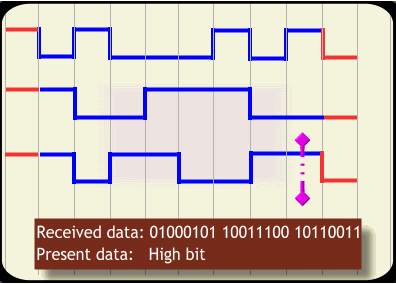
\includegraphics{serial_comm} \\
	Fonte: \href{http://electrosofts.com/parallel/}{http://electrosofts.com/parallel/}
	\label{img_serial_comm}
\end{figure}

Em seu artigo, \citeonline{Denver1995} sugere o emprego de threads para contornar possíveis problemas na comunicação serial, como a espera para receber valores. Neste caso, threads impediriam que toda uma aplicação parasse até que a transmissão deste valor seja completada. 

\section{Qt em Python}

Segundo seu criador (informação verbal, \cite{Rossum2003}), Python foi criada no início da década de 90, com influências de outra linguagem na qual trabalhara, chamada ABC. O objetivo do projeto ABC era de criar uma linguagem que pudesse ser ensinada à usuários inteligentes de computadores, mas que não eram programadores nem desenvolvedores de softwares. Após ingressar em outro projeto, surgiu a necessidade de implementação de outra linguagem, onde Rossum teve a iniciativa de criar o Pyhton: uma  linguagem simples e escalável, que permitisse a contribuição de terceiros.

Se tratando de sua arquitetura, Python é uma linguagem de alto nível, orientada a objetos e com tipagem dinâmica e forte. As definições de escopo e blocos de código são representadas por indentações, o que torna o código mais organizado e visualmente aprazível, dispensando a utilização de chaves para delimitar escopo. Além disto, permite interoperabilidade com outras linguagens. Por exemplo, utilizando a ferramenta Cython é possível, a partir de um código Python, gerar um código equivalente em C. Existem funções, inclusive, que são desenvolvidas em C, a fim de agilizar o processamento de grandes bases de dados, mas implementadas em Python.

No âmbito acadêmico, Python apresenta boas vantagens. Não só é considerada simples fácil de aprender, como é gratuita e open source. Logo, seus usuários e clientes não têm custos com licenças e seus desenvolvedores podem usar livremente códigos publicados por terceiros, que geralmente se apresentam de fácil acesso na internet, e adaptá-los às suas necessidades. Em sua enquete, \citeonline{Overflow2019} avaliou Python como a 2ª “linguagem mais amada” pelo público, atrás de Rust.

Pela facilidade de compartilhamento e comunidade crescente de usuários, existem diversas bibliotecas úteis de Python que podem ser baixadas diretamente de um repositório online e facilmente instaladas. Como alguns exemplos, cita-se as libs SQLAlchemy \cite{sqlalchemy}, que permite criação e acesso a bancos de dados leves; NumPy, uma poderosa ferramenta para cálculos matriciais \cite{harris2020array}; e PyQt5, que possui objetos e métodos para criação de interfaces gráficas \cite{pyqtdoc}.

Segundo sua documentação \cite{pyqtdoc}, a biblioteca PyQt5 veio da biblioteca de C++ “Qt”, que implementa APIs para outras linguagens, permitindo-as implementar seus objetos em seus códigos. No seu site oficial, existe uma documentação extensa de todos os seus objetos em C++, e existem também muitos exemplos disponíveis online, tanto em sites oficiais do Qt como em fóruns de programadores.

Existem 3 módulos do PyQt utilizados para criação de GUIs locais:

\begin{itemize}
	\item QtWidgets: engloba os objetos gráficos principais, como botões, textos e layouts. O objeto genérico QWidget, herdado por diversos outros deste módulo, tem funções cruciais relativas ao posicionamento, geometria, visibilidade e estilo dos objetos gráficos.
	\item QtCore: este módulo lida com eventos dos objetos da GUI, como cliques de botões e edições de caixas de texto, e conecta estes eventos com funções definidas pelo programador. Ele também permite que ele configure a aplicação principal e coordena possíveis threads iniciadas por ela.
	\item QtGui: contém objetos que possibilitam a edição de cores e bordas dos Widgets e também lida com eventos relacionados à atualização da posição e estética destes objetos.
\end{itemize}

Para iniciar a GUI, deve ser criado um objeto \emph{QApplication}, que representa o núcleo da aplicação, juntamente com as janelas da mesma, que são objetos \emph{QMainWindow}. Estes aceitam um objeto genérico \emph{QWidget} como Widget central principal (através do método \emph{setCentralWidget()}), cujas características de tamanho e layouts internos definem o tamanho da janela. Inicia-se a aplicação pelo comando \emph{exec\_()}, e as janelas pelo comando \emph{show()}.

Numa interface criada com PyQt5, os objetos visíveis dispostos na tela são chamado de Widgets, e herdam da classe \emph{QWidget}. Por conta da arquitetura em objetos da biblioteca, o desenvolvimento de supervisório didático seguiu a filosofia de incluir um objeto dentro de outro. Assim, foi possível definir melhor o espaço e as condições de redimensionamento dos objetos quando a janela for esticada ou comprimida, pois cada layout redimensiona apenas os Widgets que contém, dentro do espaço disponível.

A Figura \ref{img_exemplo_qwidget} ilustra a organização padrão de uma aplicação em PyQt, listando também alguns objetos populares.

\begin{figure}[hbt]
\centering
\caption{Janela \emph{QMainWindow} com um \emph{QGroupBox} como Widget central, contendo vários outros Widgets em um layout \emph{QGridLayout} dentro de outro layout \emph{QHBoxLayout}}
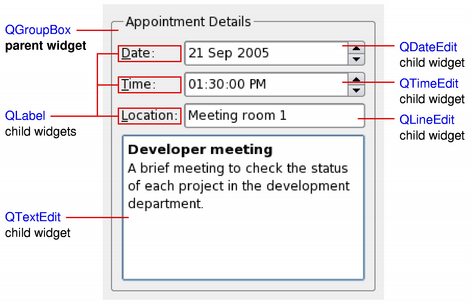
\includegraphics{Exemplo_QWidget} \\
Fonte: \href{https://doc.qt.io/qt-5/qwidget.html}{https://doc.qt.io/qt-5/qwidget.html}
\label{img_exemplo_qwidget}
\end{figure}
